\documentclass{report}


% Preamble for english writing
\usepackage[utf8]{inputenc}
\usepackage[T1]{fontenc}
\usepackage{amsmath}
\usepackage{amsfonts}
\usepackage{amssymb}
\usepackage{amsthm}
%\usepackage{algorithmic}
\usepackage{color}
\usepackage{enumerate}
\usepackage{stmaryrd}
\usepackage{hyperref}
\usepackage{graphicx}

%\usepackage{tkz-graph}

%\usepackage[nottoc, notlof, notlot]{tocbibind}

%%%%%%%%%%%%%%%%%%%%%%%%%%%%%%%%%%%%%%%%%%%%%%%%%%%%%%%%%%%%%%%%%%%
%Commandes ajoutées
%%%%%%%%%%%%%%%%%%%%%%%%%%%%%%%%%%%%%%%%%%%%%%%%%%%%%%%%%%%%%%%%%%%

%ensmembles
\newcommand{\N}{\mathbb{N}}
\newcommand{\Z}{\mathbb{Z}}
\newcommand{\Q}{\mathbb{Q}}
\newcommand{\R}{\mathbb{R}}


\newcommand{\intv}[2]{\llbracket #1, #2 \rrbracket} %intervalle d'entiers
\newcommand{\bracket}[1]{{\langle #1 \rangle}} %parenthèses angulaires
\newcommand{\gO}{\mathcal{O}} %grand O
\newenvironment{itemiz}{\renewcommand\labelitemi{$\blacktriangleright$}\begin{itemize}}{\end{itemize}}

\newcommand{\rg}{\text{rg}}
\newcommand{\bad}{\textbf{/!\backslash}}

\newcommand{\crk}{\text{cut-rank}}

\newcommand{\ie}{\emph{i.e.}\ }
\newcommand{\eg}{\emph{e.g.}\ }
\newcommand{\cf}{\emph{c.f.}\ }

% Theorems etc.
\newtheorem{Thm}{Theorem}[section]
\newtheorem{Cor}[Thm]{Corollary}
\newtheorem{Lem}[Thm]{Lemma}
\newtheorem{Pro}[Thm]{Proposition}

\theoremstyle{remark}
\newtheorem{Rem}[Thm]{Remark}
\newtheorem{Not}[Thm]{Notation}
\newtheorem{Exa}[Thm]{Example}

\theoremstyle{definition}
\newtheorem{Def}[Thm]{Definition}

\newcommand{\mytitle}[1]{
\begin{center}
\vspace{7cm}
\hrule
\vspace{0.5cm}
\huge{\textsc{#1}}
\vspace{0.5cm}
\hrule
\vspace{1cm}
\end{center}}




\title{Machine Learning Project Report\\\textbf{Evolutionnary Computing on\\Turing machines}}
\author{Jean-Florent Raymond\\\href{mailto:jean-florent.raymond.8795@student.uu.se}{\texttt{jean-florent.raymond.8795@student.uu.se}} \and Emilio Del Tessandoro\\
  \href{mailto:emilio.del_tessandoro.4062@student.uu.se }{\texttt{emilio.del\_tessandoro.4062@student.uu.se }}}
\date{\today}

\begin{document}
\maketitle

\begin{abstract}
  Busy beavers are Turing machines that performs ``the most operations'' before halting among all Turing machines with the same alphabet and number of states. Finding busy beavers becomes quickly difficult when the alphabet size and the number of states grows because of the huge number of different machines and because of the halting problem, which make us unable to know if a given machine will halt or no. Currently, busy beavers are only known for small alphabets and number of states and have only be studied by detecting ``good'' patterns on the tape or by executing different machines until it halts (if so).
  The goal of our project is to see if evolutionnary computing techiques are suitable for finding busy beaver. We deal with a population of Turing machines which can mutate an crossover. A big issue is the computation of the fitness function, since we don't know and cannot know when a machine will halt (if it halts).
\end{abstract}

\chapter{Introduction}
\label{chap:intro}

\section{Conventions}

We assume that the reader is familiar with the notion of Turing machines. In this paper, we only deal with deterministic Turing machines which have a finite alphabet and a finite set of states, so it is what we mean when we use the expression \emph{Turing machine}. Except where otherwise stated, we use the letter $m$ to denote the cardinality of the alphabet and the letter $n$ to denote the cardinality of the states set minus one (because of the halting state).

Turing machines we deal with have only one halt state. Let $\mathcal{T}_{m,n}$ be the set of deterministic Turing machines with an alphabet of $m$ symbols which uses $n + 1$ states, one of whom is the halt state, reached at most one time (because then the machine halts). Let  $\mathcal{T} = \cup_{n,m \in \N} \mathcal{T}_{n,m}$.

\section{Busy-beavers}
\label{sec:bb}

Let $s : \mathcal{T} \to \N \cup \{-1\}$ be the function which, given a Turing machine $M$, returns
\begin{itemize}
\item either the number of steps that $M$ performs when started on a blank tape, if $M$ halts ;
\item or minus one else.
\end{itemize}

\noindent And let \emph{max-step function} $S$ be defined by
\[
S : \left |
  \begin{array}{l}
    \N \times \N \to \N\\
    (m,n) \mapsto \max_{M \in \mathcal{T}_{m,n}} s(M)
  \end{array}
\right .
\]


\noindent A \emph{busy beaver} of $\mathcal{T}_{m,n}$ is a Turing machine $M \in \mathcal{T}_{m,n}$ such that \[s(M) = S(m,n)\] \ie a machine that permforms the most shifts among all machines of $\mathcal{T}_{m,n}$.

\begin{Rem}
  The functions $s$ and $S$ are not computable because otherwise it would means that we can decide the halting problem. In fact, if we assume that $s$ is computable, then the function $H : \mathcal{T} \to \{0,1\}$ such that
  \[
  \forall M \in \mathcal{T},\ H(M) =
  \left \{
    \begin{array}{l}
      0\quad \ \text{if}\ s(M) = -1\\
      1\quad \ \text{else} 
    \end{array}
  \right .
  \]
  is computable too. This function decides the halting problem, that is absurd \cite{turing}. So $s$ is not computable we can get the same result for $S$ by the same token.
\end{Rem}

\begin{Rem}
  Other definitions of busy beavers exists. For instance, we can want to find machines that leave the most symbols on the tape when halting (if so) \cite{rado}.  
\end{Rem}

% \section{Finding Machines That Reaches Bounds}

% The goal of this project is to find, at least for small values of $m$ and $n$, Turing machines that reaches $\Sigma(m,n)$ or $S(m,n)$, \ie finding a machine $M \in \mathcal{T}_{m,n}$ such that $\sigma(M) = \Sigma(m,n)$ or $s(M) = S(m,n)$.

% Such machines have already been found \cite{rado} but only for small values of $m$ and $n$ because $S$ and $\Sigma$ functions grows very fast \cite{rado}, thing that makes tests difficult.


% \paragraph{How?} This will be done using evolutionary computing techniques on a population of Turing machines coming from the same class $\mathcal{T}_{m,n}$, for fixed $m$ and $n$. The operations of crossover and mutation are made from the transition tables (the alphabet and the number of states will remain unchanged).

% After this, we also want to try an other approach using particle swarm optimization.

% \paragraph{Fitness Function}
% The main problem is to define a good fitness function. The value to maximize here is the number of steps before halting (for the max-step case), in order to reach the bound.

% Suppose we have a machine $M$ which halts after $p$ steps and a machine $M'$ which continues to run after $p$ steps.
% We cannot say that $M'$ is better than $M$ w.r.t.\ max-step, because we don't know if $M'$ will stop and we have no general way to know it (since the halting problem is undecidable \cite{turing}).
% However, for fixed $p \in \N$, we are able to say if a given machine will stop in less than $p$ steps. To know it, we simply run the machine during $p$ steps and watch if it is on a halting state at this time.

% The approach we want to try here is depends on what bound we want to reach:
% \begin{itemize}
% \item for small values of $n,m \in \N$, values of $\Sigma$ and $S$ are known \cite{rado} so a suitable fitness function is a function which, given a Turing machine $M$ that we already run on $p$ steps without leading it in the halting state, returns $- \infty$ if $p > S(m,n)$ and $\frac{1}{S(m,n) - p}$ else. With this function, Turing machines which overtake the bound are highly penalized (because we know they will never halt) and a machine which run longer (but less than $S(m,n)$) without halting than an other one get a better grade.

% \item for values of $n, m \in \N$ for which $\Sigma$ and $S$ are not known, we can, for growing values of $p \in \N$, find machines which halts after $p$ steps with a fitness function of the same kind as before. Then the more $p$ will be high, the more we will approximate the bound if we still find machines for this $p$. Note that we will probalbly not able to use this approach for many different values of $m$ and $n$ because known lower bounds for $S$ and $\Sigma$ grows very fast, what make the computations long.
% \end{itemize}

\section{Evolutionnary Computing}
\label{sec:ec}

\chapter{Strategy}
\label{chap:strategy}

\chapter{Work Organisation}
\label{chap:wo}

\chapter{Implementation}
\label{chap:impl}

\section{Turing Machine}
[...]
We implemented crossovers and mutations here since they depends on the representation of the individual type: the population method is not aware of \textit{how} we implement for example the transition table. Actually we could have some flags (like in Matlab) like: ``it is a string'', ``it is a bit string'', etc. But, since the key point of all our work are probably these two functions, we preferred to implement them where we have all the details of the individual representation, the Turing Machine.

\subsection{Crossover}
\label{sec:crossover}
[TODO Crossover implementation and assumptions, or in another chapter?]

\subsection{Mutation}
\label{sec:mutation}
[TODO Mutation implementation and assumptions, or in another chapter?]


\section{Virtual Machine}

\subsection{Fitness function}
\label{sec:fitness}
[TODO Fitness function implementation and assumptions, or in another chapter?]



\section{Evolutionary Computing Tool}
This tool has been implemented with the aim to be as general as possible; with C++ in fact is relatively easy to abstract from the type of the individuals. The implementation is inside the file \texttt{population.hpp}.

The idea behind the tool is to hide all the common operations a population method should implement. The main task of the user is to define the type of the individuals, let's say \texttt{I} (that stands for individual), and the genetic operators between individuals (that can be of many kinds). \texttt{I} can be a geometric vector, a neural network or, in our case, a living virtual machine.

In particular, except the representation of the individual, the user must define:

\begin{enumerate}
\item A fitness function. Greater values of this function means that the individual is a ``better'' solution for the problem (in other words we are trying to \textit{maximize} the fitness function). Regarding more what concerns the implementation we searches for a member function of the type \texttt{I}, in particular a function with signature \texttt{double I::fitness(I\&)}.

\item A mutation function. By default the implementation searches for a function with a signature like \texttt{void I::mutate(I\&)}\footnote{Actually the signature is slightly different because we also have as argument the reference to a random number generator. Here we explain mainly the idea.}.

\item A crossover function. We need here a function like \texttt{void I::crossover(I\&, I\&)}, that is a function that takes two individuals and modify them. In this case, if we want to keep the old individuals, we need to previously copy them.

\item (Optional) A generation function. This function is used to have additional freedom during the execution of the genetic algorithm. It's something the user can decide to do on every individual, at every generation. By default a function like \texttt{void I::generation(I\&, int)}, where the second argument is the generation number.
\end{enumerate}

We always stated ``by default'' because it's possible also to specify other user defined functions (for example not members of the \texttt{I} type). These four functions are then used in the population implementation, where needed.

The skeleton is the classical of the genetic algorithms: for every generation executes the genetic operators and then the selection.

\subsection{When to crossover and when to mutate}

The idea should be that each individual has some probability to be mutated and some probability to be crossed. The implementation of the ``with some probability'' is easy (just draw a real in $[0,1]$ and compare with a real, still in $[0,1]$, representing the wanted probability) but there are some points to clarify.

\begin{enumerate}
\item If one individual has been chosen for mutation, it can be chosen also for crossover.
\item If one individual has been chosen for crossover, which other individual choose to actually perform the crossover? [TODO explain the issue 4]
\end{enumerate}

\subsection{When to evaluate the fitness function}

Here the point is that we need a fitness value for each individual at each generation, in order to perform selection.
We thought at this problem because our fitness function is quite heavy to compute, and could happen that sometimes an individual remain unchanged from one generation to another. In this case a re-computation of the fitness function should be avoided.

So, since this is a general problem, inside the population method we used a flag to remember, for every individual, if he has been changed or not. We also save the last fitness value, that is simply a real value. If the flag says that the individual has been changed we need to re-compute the fitness function, otherwise we can use the stored result.
This optimization in some cases has shown to be very effective [TODO mention some numbers?].

\subsection{Selection}

[TODO We implemented rank selection...].

\begin{figure}[h]\centering
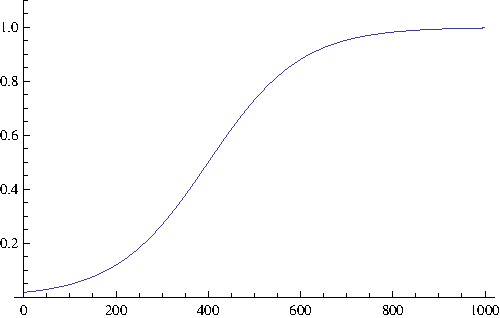
\includegraphics{figures/decision-function.pdf}
\caption{Sigmoid function used to decide if keep or not one individual. On the $x$ axis there is the individual rank. With this function the population size will average 400 individuals (maximum population size).}
\end{figure}


\section{Further work}


\chapter{Results}
\label{chap:results}

\chapter{Outcome}
\label{chap:outcome}

\bibliographystyle{acm}
\bibliography{report}

\end{document}